\subsection{Subthreshold Operation}

In the previous section, you were introduced to the structure of both n- and p-type MOSFETs and the functionality of the MIS capacitor. Let's finally have a look how to actually generate a current with out transistor. Remember from section \ref{sec:mis_capacitance_structure}, that our MOS capacitor has four different operation modes: accumulation, flatband, depletion and inversion. The modes we are interested in are depletion and inversion. 

\subsubsection{Prelude: Drift and Diffusion Current}

The current that is generated in depletion mode is caused by diffusion and we say that we operate in the subthreshold or weak inversion regime. On the other hand, the current generated in inversion mode is caused by drift and we say that we operate in the superthreshold or strong inversion regime. Let's recap what exactly drift and diffusion currents are.\\

A drift current is caused by an applied electrical field. The field's electrical force defines the strength and direction into which charged particles are pulled. As equally charged particles repel each other and are attracted to opposite charges, negatively charged particles are pulled towards the more positive side of the field and vice versa. Due to the generated movement of charges, we get a current. This current is defined by the following equation:

\begin{equation}
    I = q n \mu \epsilon
\end{equation}

where $q$ is the electron charge, $n$ the carrier density, $\mu$ the carrier mobility and $\epsilon$ the electrical field. This mechanism is also visualized in figure \ref{fig:drift_current}. An electron is pulled towards a point with lower electron energy, i.e. voltage. On the other hand, a hole is pulled towards a point with higher voltage. The slope corresponds to the electrical field $\epsilon$.\\

\begin{figure}
\centering
\begin{subfigure}{.5\textwidth}
  \centering
  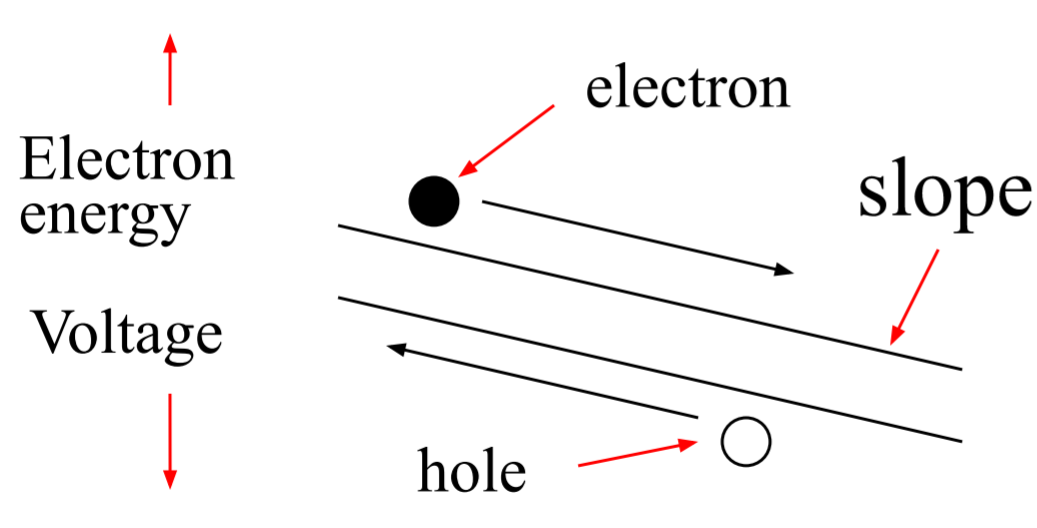
\includegraphics[width=\linewidth]{Figures/drift_current.PNG}
  \label{fig:drift_current}
\end{subfigure}%
\begin{subfigure}{.5\textwidth}
  \centering
  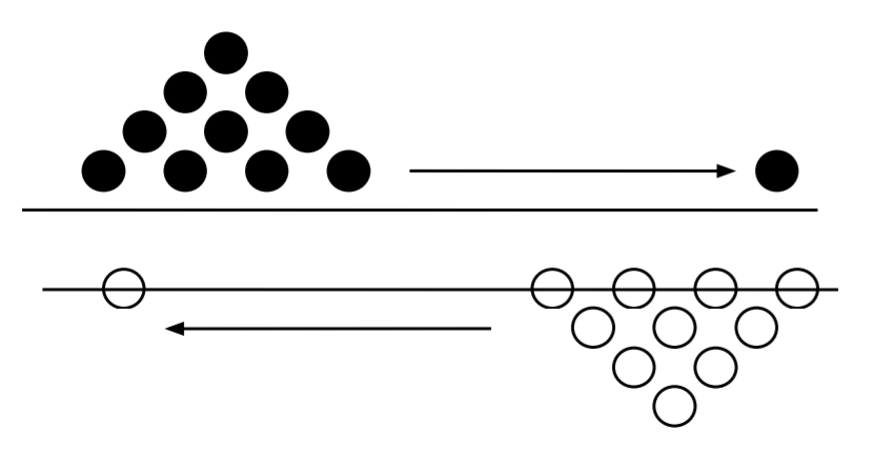
\includegraphics[width=\linewidth]{Figures/diffusion_current.PNG}
  \label{fig:diffusion_current}
\end{subfigure}
\caption{The concept of drift (left) and diffusion (right) current.}
\end{figure}

A diffusion current is caused by a difference in concentration. We experience diffusion on a daily basis, for example when dipping our tea bag into hot water and seeing it spread or when watching the smoke of a nearby factor that diffuses into the air. Diffusion describes the movement from a region of higher concentration to a region of lower concentration. In our case, this movement of charged particles generates a current which can be described as follow:

\begin{equation}
    I = -q D \frac{dN}{dz}
\end{equation}

where $q$ is the electron charge, $D$ the diffusion constant and $\frac{dN}{dz}$ the concentration gradient. The higher the concentration difference, the higher the resulting current. The concepts of diffusion is also visualized in \ref{fig:diffusion_current}.\\

It is important to note that in both regimes diffusion \textbf{and} drift current occur. However, in subthreshold the electric field is so weak that it can be neglected next to the diffusion current and vice versa. As you have seen previously, the mode we operate in depends on our gate voltage and we switch from the sub- to the superthreshold regime once our gate voltage crosses a threshold voltage at which point electrons become the majority carriers assuming a p-type channel.\\

\begin{figure}
    \centering
    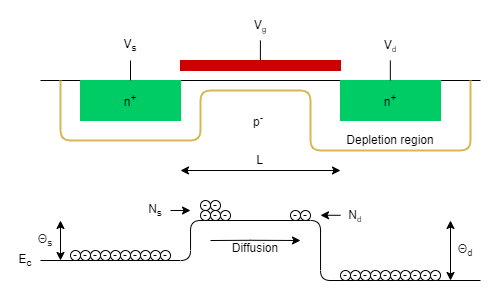
\includegraphics[width=.8\linewidth]{Figures/subthreshold_diffusion_energy.png}
    \caption{nFET MOSFET structure and its corresponding conduction band.}
    \label{fig:nfet_diffusion_energy}
\end{figure}

Let's have a look at our MOSFET when we don't apply any gate voltage. For the following derivations we assume an n-type MOSFET. Remember that an nFET consists of a p-type body and an n-type source and drain. Figure \ref{fig:nfet_diffusion_energy} visualizes an nFET transistor and its conduction band $E_c$. At the contact points between the n-type source and drain with the p-type body, we have a pn-junction. As introduced in section \ref{sec:pn_junction_diode}, the conduction band of the p-type has a higher electron energy than the conduction band of the n-type. This energy difference creates a barrier between the source and the drain that prevents any current from flowing. We denote this energy difference the built-in potential $\Theta_0$. It is the energy an electron requires to move from the n- to the p-type.\\

What happens to our energy barrier as soon as we increase the gate voltage? The positive charge at the gate repels the free holes in the p-substrate and a region with only fixed negatively charged ions, the depletion region, remains. As introduced in section \ref{sec:mis_capacitance_structure}, the charge of this region is defined by its surface potential $\psi_s$. By adding an external voltage to the p-type, we lower its conduction band and therefore decrease our energy barrier. On the other side, remember that our source and drain are also connected to an external voltage $V_s$ and $V_d$. These allow us to change the conduction band of the n-type source and drain, and consequently the energy barrier, as well. We can therefore describe the height of the energy barriers at the source and the drain as follows:

\begin{equation}
    \Theta_s = \Theta_0 - q \psi_s + q V_s = \Theta_0 - q (\psi_s - V_s)
\end{equation}

\begin{equation}
    \Theta_d = \Theta_0 - q \psi_s + q V_d = \Theta_0 - q (\psi_s - V_d)
\end{equation}

We assume that the surface potential $\psi_s$ along the channel is constant. Note that $V_s, V_d \ge 0$ in order to keep our transistor reverse biased, so we cannot simply add a negative voltage to our source and drain to decrease the energy barrier. The height of the energy barrier determines how many electrons can diffuse from the n-type to the p-type channel. The electron densities at the edges of the p-type channel can be described by the following equation:

\begin{equation}
    N_s = N_0 e^{-\Theta_s/kT}
\end{equation}

\begin{equation}
    N_d = N_0 e^{-\Theta_d/kT}
\end{equation}

As expected, the carrier density increases exponentially for a decreasing energy barrier. It should be clear now why we need $V_d > V_s$ for a current to flow. If $V_d = V_s$, $N_d = N_s$ and there is no change in carrier concentration across the channel and hence no diffusion current. For increasing values of $V_d$, we increase the energy barrier on the drain side of the channel which leads to smaller concentration of electrons. The concentration gradient between the source and the drain can simply be described by:

\begin{equation}
    \frac{N}{dz} = \frac{N_s - N_d}{L}
\end{equation}

where $L$ is the length of the channel. In a semiconductor, the diffusion current is given by:

\begin{equation}
    I = -q W t D_n \frac{dN}{dz}
\end{equation}

where $D_n$ is the diffusion constant, $W$ the width of the channel and $t$ the depth of the channel. By inserting the retrieved formula for our concentration gradient, we finally get the equation for our subthreshold current:

\begin{equation}
    I_{ds} = -q \frac{W}{L} t D_n (N_d - N_s) = -q \frac{W}{L} t D_n e^{\frac{\psi_s}{U_T}} (e^{\frac{-V_d}{U_T}} - e^{\frac{-V_s}{U_T}}) = I_0 e^{\frac{\psi_s}{U_T}} (e^{\frac{-V_s}{U_T}} - e^{\frac{-V_d}{U_T}})\label{eq:sub_ids_psi}
\end{equation}

where $I_0 = q \frac{W}{L} t D_n N_0 e^{\frac{-\psi_0}{U_T}}$ is the so-called leakage current. It can be easily extracted in an experimental setup by setting the voltage difference between the gate and the source to zero, i.e. $V_{gs} = 0$, and measuring the remaining current. The problem with \eqref{eq:sub_ids_psi} is that it depends on the surface potential $\psi_s$ that we cannot directly control. However, as introduced in section \ref{sec:mis_capacitance_structure}, $\psi_s$ is related to the gate voltage $\V_g$ via:

\begin{equation}
\frac{\Delta \Psi_s}{\Delta V_g} = \frac{C_{ox}}{C_{ox} + C_{dep}} := \kappa
\end{equation}

Substituting this relationship into \eqref{eq:sub_ids_psi} yields:

\begin{equation}
    I_{ds} = I_0 e^{\frac{\kappa V_g}{U_T}}(e^{\frac{-V_s}{U_T}} - e^{\frac{-V_d}{U_T}}) \label{eq:fullsubcurrent}
\end{equation}

We denote the current $I_{ds}$ as the current flow from the drain to the source. Note that current flows \textbf{in the opposite direction} of the electrons. When rewriting \eqref{eq:fullsubcurrent}, we see that the subthreshold current $I_{ds}$ actually consists of two components: the current from the drain to the source of the transistor, the so-called forward current, minus the current from the source to the drain of the transistor, the so-called reverse current.

\begin{equation}
    I_{ds} = I_0 e^{\frac{\kappa V_g - V_s}{U_T}} - I_0 e^{\frac{\kappa V_g - V_d}{U_T}} = I_f - I_r
\end{equation}\\

We can further rewrite the current equation as follows:

\begin{equation}
    I_{ds} = I_0 e^{\frac{\kappa V_g - V_s}{U_T}} (1 - e^{\frac{-V_{ds}}{UT}}) \label{eq:satsubcurrent}
\end{equation}

where $V_{ds}$ is the voltage difference between the drain and the source $V_d - V_s$. We can see that for large values of $V_{ds}$, the reverse current of the equation eventually becomes negligible. When this happens, we are said to operate in the saturation region. The regime in which both the forward and the reverse current shape $I_{ds}$ is called the triode, linear or ohmic region. The point at which we move from the linear to the saturation regime is approximately at $V_{ds} = 4 U_T \approx 100 mV$. The relationship between $V_{ds}$ and $I_{ds}$ is also visualized in figure \ref{fig:vsd_vs_ids} for different values of $V_{gs}$. Note that all values of $V_{gs}$ are in subthreshold and it only influences the strength of the resulting current.\\

\begin{figure}
    \centering
    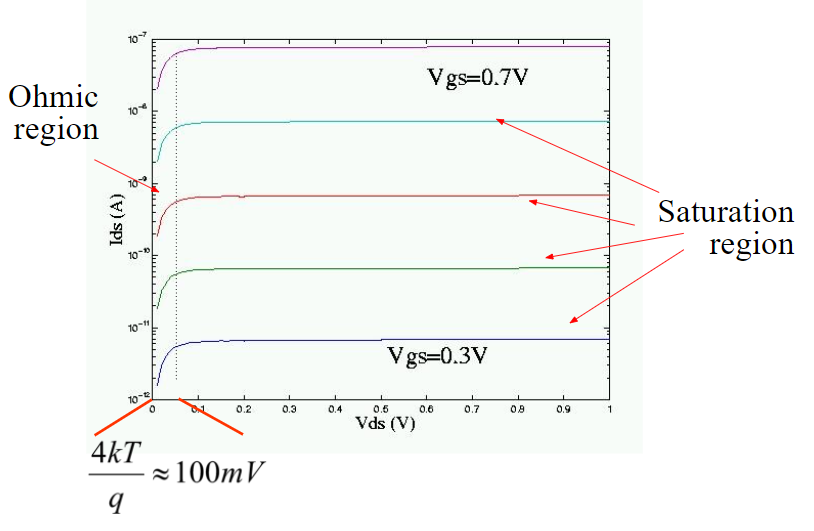
\includegraphics[width=.8\linewidth]{Figures/Vds_vs_Ids.PNG}
    \caption{Relationship between the drain-to-source voltage $V_{ds}$ and the current $I_{ds}$.}
    \label{fig:vsd_vs_ids}
\end{figure}

Let's sum up the equations we derived for an nFET transistor in the subthreshold regime.\\

\textbf{Subthreshold nFET $I_{ds}$ current}
\begin{itemize}
    \item Triode/ Linear/ Ohmic Region
    \begin{equation}
        I_{ds} = I_0 e^{\frac{\kappa V_g - V_s}{U_T}} (1 - e^{\frac{-V_{ds}}{UT}}) = I_f - I_r
    \end{equation}
    \item Saturation Region
    \begin{equation}
        I_{ds} = I_0 e^{\frac{\kappa V_g - V_s}{U_T}} = I_f
    \end{equation}
\end{itemize}